\chapter{Experimental Results}

\label{ch:results}

TODO: Re-adapt this text into a dissertation chapter!!

\begin{quote}
\dunyazad/ is a system which constructs narrative choices a la Choose-Your-Own-Adventure books.
%
It constructs choices -- including the setup, the options, and the outcome for each option -- to achieve specific poetic effects, that is, to control how players perceive the choices it generates.
%
This paper demonstrates \dunyazad/'s ability to manage player expectations by having it generate three distinct choice structures: obvious choices, relaxed choices, and dilemmas.
%
Because it uses answer set programming, \dunyazad/'s choice generation system not only generates choices, but itself constitutes a first-order theory of choice poetics.
%
Survey data presented here thus not only validate that players' perception of choices matches \dunyazad/'s intended poetic effect, but also inform the theory of choice poetics.
%
Statistical analysis of our data indicates that \dunyazad/ can successfully construct obvious choices, relaxed choices, and dilemmas.
\end{quote}


\section{Introduction}

\dunyazad/ is a novel interactive story generation system which generates choices in the style of Choose-Your-Own-Adventure novels.
%
One of its primary goals is to generate individual choices that achieve specific poetic effects.
%
For example: generating a choice that makes the player feel anxious.
%
To generate choices, it creates framing situations (e.g., ``A dragon is attacking you.''), assembles a range of primitive actions (e.g., ``flee''), determines their arguments (e.g., ``You flee from the dragon.'' vs. ``The dragon flees from you.''), and assigns them consequences (e.g., ``You cannot escape. The dragon eats you.'').
%
By a conservative estimate, there are tens of thousands of choice configurations that \dunyazad/ could generate when accounting for variation in the framing, options, and outcomes of a choice.
%
An example of a choice generated by \dunyazad/ is presented in \cref{fig:exchoice}.


To exercise \dunyazad/'s player expectation system, we set it up to construct three different types of choices:
%
\begin{itemize}
  \item \emph{Relaxed} choices, where the stakes were low and there were no bad options.
  \item \emph{Obvious} choices, where there was a single option that stood out as more advantageous than the rest.
  \item \emph{Dilemmas}, where every option was about equally undesirable.
\end{itemize}
%
Being able to construct these types of choices relies heavily on modelling players' expectations, so if the system can do so successfully, it shows that its models of player expectations are working.
%
This capability is important for a system that wants to manage choice poetics, and in fact player perceptions of a choice such as ``This choice has no bad options,'' or ``This choice has a clear best option,'' are themselves choice poetics.
%
These simple poetics contribute to more complicated reactions like ``This choice feels relaxed,'' so getting them right is important for \dunyazad/.
%
Although the system has some components that reason about more complicated poetics, the goal of this study was to verify the core expectation-tracking capabilities.


To test the system's performance, we ran a survey that asked participants to read a single choice generated by the system and answer some questions about their perception of the choice.
%
Each participant saw one of the three categories of choices, and our data analysis compares the responses across categories and against a uniform distribution to determine if players' perceptions match what the system intended.
%
Our data show that \dunyazad/ was mostly able to achieve what it set out to, although in a few specific cases there were surprising results.
%
Because \dunyazad/ is a transparent operationalization of choice poetic theory, however, both the expected and surprising results can usefully inform not only the system's construction but also the theory of choice poetics.

\begin{figure}[h]
\fbox{
\parbox{0.95\columnwidth}{
  \slshape
You come to a tavern and decide to rest for a while. 
%
A merchant is bored and a noble is bored and an innkeeper seems knowledgeable. 
%
What do you do?
\begin{enumerate}[itemsep=0pt,topsep=4pt,parsep=0pt,partopsep=0pt]
\item You play a song for the noble \\
  (You have skill: musician. You have no tool for music).
\item You gossip with the innkeeper \\
  (You are missing skill: negotiation).
\item You play a song for the merchant \\
  (You have skill: musician. You have no tool for music).
\end{enumerate}
}
}
  \caption{An example choice.}
  \label{fig:exchoice}
\end{figure}


\section{Related Work}

This study is part of a recent trend focusing on choices in narrative, and several groups have published interesting results.
%
In 2011, Thue, Bulitko, Spetch, and Romanuik demonstrated \work{PaSSAGE}'s ability to increase player perceptions of agency by selecting content that players liked more \citep{Thue2011}.
%
This study demonstrated a link between desirable content and perceptions of agency.
%
The \work{PaSSAGE} system itself does directly construct choices, however, nor does it consider choice poetics in its operation.
Instead, it uses online player modelling to determine what kinds of content a player prefers, and selects from pre-written quest alternatives based on that.


Fendt, Harrison, Ware, Cardona-Rivera, and Roberts showed that direct feedback after players make a choice can create an illusion of agency, albeit in an extremely simple interactive narrative \citep{Fendt2012}.
%
In this study, the choices were part of a hand-written adventure game, whereas \dunyazad/ generates choices on its own.
%
This study concentrated on how different choice structures (mainly in terms of outcome text) affected players' perceptions of agency.


In a similar study, Cardona-Rivera, Robertson, Ware, Harrison, Roberts, and Young found that choices where the options lead to significantly divergent outcomes increase feelings of agency relative to choices with similar outcomes \citep{Cardona-Rivera2014}.
%
Again this study used hand-written content as the test material; it focused on the connections between agency and divergence of outcomes.


In another study using the Choose-Your-Own-Adventure format, Yu and Riedl were able to predict and influence players' choices using collaborative filtering \citep{Yu2013}.
%
Like the Fendt et al. and Cardona-Rivera et al. studies, this study used hand-written text, but this study chose to adapt two existing Choose-Your-Own-Adventure books for their study, rather than creating their own stories.
%
This resulted in much more complex and sophisticated stories, which more closely mimics the actual conditions of entertainment consumption.
%
Yu and Riedl's system did not generate options, however, it simply selected which options to present at a choice out of a number of hand-written alternatives that conveyed different motives for choosing a particular path.
%
This is a form of choice construction (since the exact options are dynamic) but the framing and outcomes are not dynamic and the options themselves are not constructed by the system but merely selected.

Nevertheless, Yu and Riedl succeeded in using collaborative filtering to predict which of several motivations for taking the same action would be most appealing to players, and they were able to use a drama manager to guide players' choices.
%
Although their system only focused on guiding each player towards content that the collaborative filtering predicted that player would enjoy, one could imagine a more complex version that might try to influence players' perceptions of the choices themselves.
%
In contrast to Yu and Riedl's system, \dunyazad/ uses a logical model of player expectations that includes authorial input. 
%
While collaborative filtering allows a system to make user-specific adjustments and potentially allows fine-grained discrimination of player preferences, it is also quite opaque.
%
\dunyazad/'s logical model, while not adaptive, is more useful for informing a theory of choice poetics, and as our results demonstrate, it gets the job done.
%
That said, the use of online player data is something highly desirable for a system like \dunyazad/, and implementing something like Yu and Riedl's collaborative filtering is a tempting direction for future work.


These studies are mostly focused on a single particular aspect of choice poetics (such as agency) whereas \dunyazad/ attempts to address constructing poetic choices more broadly.
%
Additionally, none of the studies mentioned thus far involved narrative generation systems that construct stories from raw material.
%
Considering constructive systems that are similar to \dunyazad/, Szilas' \work{IDtension} and El-Nasr's \work{Mirage} both stand out as interactive narrative systems rooted in theories about how narrative works \citep{Szilas2003,El-Nasr2007}.
%
\work{IDtension} is based on traditional dramatic theory (i.e., normal poetics) whereas \work{Mirage} incorporates theories of drama in the theatrical sense.
%
\dunyazad/ is also guided by a narrative theory: it is based on choice poetics--the theory of how choices are perceived by an audience \citep{Mawhorter2014}.
%
In this paper, we focus on \dunyazad/'s ability to generate individual choices that manipulate player expectations--obvious choices, relaxed choices, and dilemmas.
%
In some ways, this is reminiscent of recent narrative generation systems that have focused on specific traditional poetic effects, such as \work{Suspenser} (focused on suspense) and \work{Prevoyant} (focused on foreshadowing) \citep{Cheong2006,Bae2008}.


\section{\dunyazad/}

This section gives a brief overview of how \dunyazad/ functions.
%
% TODO: Change this!!
For a more detailed description of \dunyazad/, consult \citep{Mawhorter2015}.
%
For this study, \dunyazad/ was asked to construct individual choices, rather than entire stories.
%
It uses an answer set solver (specifically the Potassco Labs tool \clingo/) to satisfy a complex set of constraints.
%
The resulting answer sets correspond to choices, each complete with a setup, several options, and the outcomes of those options.
%
In effect, \dunyazad/ searches over all possible choices as dictated by its constraints and arbitrarily picks one (subject to the whims of the solver).


Internally, \dunyazad/ uses a representation similar to the situation calculus \citep{McCarthy1963}.
%
The system can express states of and relations between characters and items in a scene, and some states and relations represent potential actions rather than immediate facts (e.g., the \texttt{selling} relation represents that a vendor is \textsl{willing to} trade an item).
%
Within the context of a single choice, there is a single starting situation, and each option leads to a modified situation based on its outcomes (unlike the original situation calculus, two different actions can lead to the same outcome situation if their effects on the state of the world are identical).
%
For the purposes of this experiment, outcome situations are irrelevant, because they are never shown to participants.
%
However, the system's understanding of what each action \textsl{might} and \textsl{will probably} do is important.
%
One of the main constraints on the system is expressed in terms of the system's understanding of player goals, which depends on its understanding of how different actions might impact those goals.
%
This player expectation subsystem is the focus of the study reported here.


When assembling a choice, \dunyazad/ makes use of a complex set of rules constraining what actions are reasonable given the story situation.
%
For example, when being threatened by a dragon, fleeing from it and attacking it are both reasonable options, but bribing yourself, casually travelling onwards, and trading with a nearby merchant are not.
%
The common-sense rules that enforce these distinctions are the ``basic plot model'' and are unfortunately too numerous to describe here in detail.
%
They include the preconditions of actions, rules about the priorities of different problems and opportunities, and some constraints over multiple options at a choice (such as rules that prevent the generation of two identical options).


Given a reasonable basic plot model, \dunyazad/ could construct choices that make sense from a narrative perspective.
%
But \dunyazad/'s goal is to construct choices that not only make sense, but which achieve specific poetic effects.
%
To this end, it must have some idea of how players perceive the options it generates.
%
Much like a human author, \dunyazad/ does not have direct access to the actions and reactions of its readers (this is by design).
%
Instead, \dunyazad/ makes guesses about its readers' goals and perceptions, and then uses textual hints to reinforce those guesses as best it can.


The root of \dunyazad/'s reasoning about player perceptions is its assumed player goals.
%
The system assumes that players will have the following goals while playing:
%
\begin{itemize}
  \item Avoid injury to their character (important).
  \item Avoid threats to their character (important).
  \item Diffuse threats to other innocent characters (important).
  \item Succeed at actions they initiate.
  \item Acquire tools for skills that they have.
\end{itemize}
%
In situations that involve one or more ``important'' goals, those goals are assumed to have priority.
%
Each choice is also determined to be ``high-stakes,''  ``low-stakes,'' or ``no-stakes'' depending on whether it involves one or more important goals, no important goals (but some non-important goals), or no player goals at all.
%
With this model of player goals, the system can calculate how each option affects them.


When considering how players perceive options, the system focuses on their potential and probable outcomes.
%
Each action in \dunyazad/ can have multiple outcome variables, each of which takes on one of several values.
%
For example, the \texttt{attack} action has a \texttt{success} outcome variable that can take on values of \texttt{victory}, \texttt{defeat}, or \texttt{tie}.
%
Effects of an action are usually predicated on particular outcomes, for example the outcome \texttt{success=victory} for an \texttt{attack} action has a consequence of removing any \texttt{threatening} relations between the defeated party and any actors they were threatening before the attack.
%
\dunyazad/ can thus understand that an option to attack someone who is threatening the player character might achieve their goal to avoid being threatened.


Particular outcomes are influenced by certain skills, for example the \texttt{success=victory} outcome of the \texttt{attack} action is influenced by the \texttt{fighting} skill of both the attacker and the defender, as well as whether those parties have tools for that skill (i.e., weapons).
%
Given the skills of the actors involved, \dunyazad/ can determine that some outcomes are \emph{likely} or \emph{unlikely} (and by manipulating which characters have which skills in the setup, \dunyazad/ can control this).
%
Consequently, the system assigns several relations between each option and each player goal:
\begin{itemize}
  \item An option ``threatens'' a goal if any possible outcome results in a state that hinders that goal.
  \item An option ``enables'' a goal if any possible outcome results in a state that advances that goal.
  \item An option ``fails'' a goal if a \emph{likely} outcome results in a state that hinders that goal.
  \item An option ``achieves'' a goal if a \emph{likely} outcome results in a state that advances that goal.
  \item Otherwise, an option is ``irrelevant'' to a goal.
\end{itemize}
The system also evaluates the player's projected perception of the actual outcomes of each option, but that is not relevant to this study.


Of course, a single option might ``enable'' one goal and ``threaten'' another, or even both ``enable'' and ``fail'' the same goal.
%
Also, individual options have to be considered together when thinking about the impact of an entire choice.
%
By placing constraints on the mix of player expectations engendered by each option at a choice, the system is able to construct ``obvious,'' ``relaxed,'' and ``dilemma'' choices.
%
The system can create a total of 14 different choice structures including ``mysterious,'' ``uncomfortable,'' and ``bleak'' choices, but only the ``obvious,'' ``relaxed,'' and ``dilemma'' structures were tested in this study.


\label{page:choicetypes}

The system's definitions for ``obvious,'' ``relaxed,'' and ``dilemma'' choices are as follows:
%
\begin{itemize}
  \item For ``obvious'' choices, there should be exactly one option which is expected to ``achieve'' a player goal and not ``fail'' any player goals, while no other option should be expected to ``achieve'' any player goal, and all other options should at least ``threaten'' a player goal.
  \item For ``relaxed'' choices, each option must at least be expected to ``enable'' if not ``achieve'' a player goal, and none may ``threaten'' or ``fail'' any player goals. Additionally, the choice should be low-stakes according to the goal priorities involved.
  \item For ``dilemma'' choices, all options should be expected to at least ``threaten'' if not ``fail'' a player goal, and those goals should all have the same priority. No option should be expected to ``achieve'' any player goal, and options that are expected to ``enable'' a player goal must also be expected to ``fail'' some goal.
\end{itemize}
%
Note that ``obvious,'' ``relaxed,'' and ``dilemma'' are author-assigned labels: they represent what the system author thinks the resulting choices will be like, but they may not be accurate.
%
The actual qualities of these choice structures don't necessarily align with their internal labels, and only with data (like those presented here) can such a correspondence be established.


Once the answer set for a choice is generated, \dunyazad/ uses a template-based natural language generation system to generate text for that choice.
%
This text (cf. \cref{fig:exchoice}) conveys the setup and potential states at a choice and includes text in each option mentioning any relevant skills and/or tools.
%
Mentioning skills/tools like this is a way for the system to explicitly encourage players to view those things as relevant.

\section{Method}

The primary goal of the experiment we conducted was to assess \dunyazad/'s ability to manage and predict player expectations.
%
To that end, we focused on players perceptions of options at a choice, and did not address issues like whether outcomes matched options.
%
The three choice types we generated were chosen because they are each distinct in terms of the player expectations they engender, and because together they cover a range of different player expectations.


To gather data on player expectations, we generated choices using \dunyazad/, showed them to study participants, and asked participants a series of questions about specific qualities of the choice they just read.
%
Because we used Amazon Mechanical Turk to gather data, our participants were each paid a small amount and presumably approached the survey as a means to earn money rather than a voluntary undertaking.
%
Because of this, questions were asked in a hypothetical manner (e.g. ``If you were reading this story, which option would you choose?'') rather than directly (e.g. by having participants pick an option) to imply that the task at hand was asking them to judge the choice as someone reading it for entertainment might.
%
Of course, this framing (and being asked specific questions in general) might encourage an analytical mode of engagement, which is not what \dunyazad/ is designed to support, but that limitation is to some degree inevitable when survey responses are solicited.


To control for participants paying little attention, being unfamiliar with English, or simply filling in random responses, two check questions were asked.
%
Responses from participants who failed to answer these questions satisfactorily were excluded from the analysis, as were responses where one or more questions were left blank (about 15\% of all participants).

\subsection{Treatments}

For this experiment, there were three experimental treatments, each corresponding to a different set of rules used by \dunyazad/ to generate the choice experienced by a subject.
%
These are the ``obvious,'' ``relaxed,'' and ``dilemma'' choice types described on page \pageref{page:choicetypes}.
%
The system definitions given in that section represent extra constraints placed on the choices generated by \dunyazad/ beyond its common core rules.
%
Each participant thus saw a choice shaped by one of three different constraint sets.


Of course, each constraint set can generate a potentially large range of specific choices, but this study was interested in perceptions common across choices generated using the same constraints.
%
One possibility would be to show each participant a unique choice from the space of choices possible given one of the treatment conditions.
%
However, this setup would mean that no single choice would be seen by more than one participant, and so there would be no way to analyze the contribution of individual choices to the perception of the different treatments.
%
Instead, we generated three different choices per treatment, and showed each choice to ten participants.

\subsection{Setup}

To set up the experiment, we used \dunyazad/ in its ``experiment'' mode (which causes it to generate only a single choice and to use a special framing) to generate three choices for each of the experimental conditions.
%
As an additional constraint, each choice was required to have exactly three options, so that the number of options wasn't a confounding factor in our data.
%
These nine choices were generated sequentially by the system, so there was no opportunity to cherry-pick ``good'' examples of each treatment category.
%
The choice shown in \cref{fig:exchoice} is the first choice that was generated; it is in the ``dilemma'' treatment.
%
The framing for each choice presented the skills that the system had assigned the player character for that choice, and established a basic context for the choice (see \cref{fig:exframing}).
%
The framing for each choice differed only in the skills presented and the fictional destination name, which \dunyazad/ chooses randomly from a fixed list of made-up names.


\begin{figure}[h]
\fbox{
\parbox{0.95\columnwidth}{
  \slshape
You are about to set out on an epic journey. You are are heading towards towards the distant country of Jyv\"asky, hoping to earn fame and fortune.
%
You have some perfume and a book of legends, and you have skill: literacy, you have skill: musician, and you have skill: healing. 
%
Eager to be on your way, you set off on the road towards Jyv\"asky.
}
}
  \caption{Example framing.}
  \label{fig:exframing}
\end{figure}


Once the choices were generated, their text was broken into parts and put into a comma-separated values file for upload to Amazon Mechanical Turk where the parts would be substituted into a template.
%
Given a survey template, Mechanical Turk generated individual survey pages for each question, and ten tasks were posted per question (a total of 90 tasks), which workers on Mechanical Turk were able to preview, accept, and fill out for payment (50 cents per task\footnote{This was chosen based on online advice to pay about minimum wage for tasks on Mechanical Turk. Given the median response time, the hourly pay rate was \$7.50, but in retrospect, the inconvenience of survey tasks (where a worker cannot complete the same task many times and thus work more efficiently) suggests that a higher pay rate would be appropriate. If we do a similar survey in the future, we plan to pay at least twice as much, as the total cost (about \$50 in this case counting Amazon's 10\% fee) was not high.}).
%
Myle Ott's ``uniqueturker'' script (\url{https://uniqueturker.myleott.com/}) was used to ensure that no individual worker filled out the survey more than once.
%
To avoid being targeted by bots, the tasks required workers with a 97\% acceptance rate across at least 1000 accepted tasks.

\subsection{Survey Content}

Each survey was divided into three sections.
%
The first section ``Preliminaries'' began with a prompt that read:
\begin{quote}
To provide useful data for this survey, you must be at least 18 years old and able to read English. To confirm this (and to confirm that you aren't a bot), please answer the following question.
\end{quote}
%
This section just contained the following question designed to ensure that subjects were at least 18 years old and has basic English proficiency:
%
\begin{quote}
If you're at least 18 years old, please don't write ``Age of years eighteen least at am I that confirm I,'' as the answer here, instead write that sentence backwards, ended with an exclamation point. If not, please do a different HIT, as I cannot use your data in my results, and thus I will not accept your response.
\end{quote}


The second section was titled ``The Choice'' and began with a prompt:
%
\begin{quote}
Please read the following short story which presents you with a choice, then answer the questions about that choice below.
\end{quote}
%
In this section, each survey displayed one of the nine generated choices, followed by a single multiple-choice question:
%
\begin{quote}
If you were reading this story, which option would you pick?
\end{quote}
%
This question had three options: ``Option 1,'' ``Option 2,'' and ``Option 3.''


The final section of the survey was titled ``Opinion Questions'' and began with a prompt:
%
\begin{quote}
Please rate your agreement with the following statements, from 1 (strongly disagree) to 5 (strongly agree).
\end{quote}
%
This section contained the following 8 Likert items in this fixed order\footnote{These were individual Likert items which did not compose a Likert scale, as the goal of the survey was to directly measure opinions, and there were no underlying psychological variables presumed to be giving rise to behavior.} (the quotes were part of the survey):
%
\begin{enumerate}
  \item ``There are no bad options at this choice.''
  \item ``There is a clear best option at this choice.''
  \item ``The stakes for this choice are low.''
  \item ``There are no good options at this choice.''
  \item ``All of the options at this choice are about equally promising.''
  \item ``There are options at this choice.'' (This is a trick question to test whether you're paying attention. Please simply indicate that you are in complete disagreement.)
  \item ``This is a difficult choice to make.''
  \item ``This choice feels like it will have important consequences.''
\end{enumerate}
%
Each question in this section the same five numbered options presented vertically:
%
\begin{enumerate}
  \item strongly disagree
  \item somewhat disagree
  \item neutral
  \item somewhat agree
  \item strongly agree
\end{enumerate}
%
For these questions (and the multiple-choice question in the previous section) participants selected an option by clicking a radio button next to that option. There were no default responses, so someone who didn't click any of the radio buttons would submit a blank response for that question.
%
Responses were treated as ordinal data, and labeled with the numbers 1 through 5 in the same order they appeared here (i.e. 1 $\rightarrow$ strongly disagree; 5 $\rightarrow$ strongly agree).

\subsection{Hypotheses}

Before conducting the survey, we came up with a set of initial hypotheses about how participants would answer these questions based on the treatment conditions.
%
There were three types of hypothesis: single-treatment hypotheses, between-treatment hypotheses, and stakes hypotheses.
%
Each singe-treatment hypothesis posited that under a particular treatment, respondents would generally agree with or disagree with a particular question.
%
Agreement with a question was determined by a one-sided Mann-Whitney-Wilcoxon U test \citep{Mann1947,Wilcoxon1945} against a uniform distribution of responses with the alternate hypothesis being ``The median of the survey responses is significantly higher than the median of the uniform distribution.''
%
Disagreement likewise used a Mann-Whitney-Wilcoxon U test with the alternate hypothesis that the median of the survey responses was smaller than that of a uniform distribution.
%
In both cases, a confirmation of a hypothesis was taken to be significant for $p < 0.05$.


\begin{table}
\bgroup
\def\arraystretch{1.1}
\begin{tabular}{l | l | l | l |}
Question & Obvious & Relaxed & Dilemma \\
\hline
1 &     -    &  agree   & disagree \\
\hline
2 &  agree   &     -    & disagree \\
\hline
3 &     -    &  agree   &     -    \\
\hline           
4 & disagree & disagree &  agree   \\
\hline
5 & disagree &     -    &  agree   \\
\hline
6 &     -    &     -    &     -    \\
\hline
7 & disagree &     -    &  agree   \\
\hline
8 &     -    &     -    &  agree   \\
\hline
\end{tabular}
\egroup
  \caption{Initial single-treatment hypotheses by treatment.}
  \label{tab:single-treatment}
\end{table}


For the between-treatment hypotheses, survey data from two different treatments were compared using a Mann-Whitney-Wilcoxon U test to test whether one was statistically more-agreed-with than another (with the threshold for significance again being set at $p < 0.05$).
%
The statistics are the same for the converse cases, so only one test was performed per hypothesis (i.e., if responses to question 3 showed significantly more agreement for the ``obvious'' treatment than for the ``relaxed'' treatment, it follows automatically that they show significantly less agreement for the ``relaxed'' treatment than for the ``obvious'' treatment).
%
The single-treatment hypotheses are shown in \cref{tab:single-treatment} while the between-treatment hypotheses are shown in \cref{tab:between-treatments}.
%
Across all 3 treatments, there were a total of 13 single-treatment and 9 between-treatment hypotheses.


\begin{table}
\bgroup
\def\arraystretch{1.1}
\begin{tabular}{p{3.5em} | p{5em} | p{5em} | p{5.5em} |}
Question & Obvious & Relaxed & Dilemma \\
\hline
1 &      -     & $>$Dilemma &      -     \\
\hline
2 & $>$Dilemma &      -     &      -     \\
\hline
3 &      -     &      -     &      -     \\
\hline
4 &      -     &      -     & $>$Both Other \\
\hline
5 &      -     &      -     & $>$Obvious \\
\hline
6 &      -     &      -     &      -     \\
\hline
7 &      -     &      -     & $>$Both Other \\
\hline
8 &      -     &      -     & $>$Both Other \\
\hline
\end{tabular}
\egroup
  \caption{Initial between-treatment hypotheses by treatment. The ``$>$'' signs indicate more agreement relative to the alternate treatment indicated. ``$>$Both Other'' indicates that that treatment is hypothesized to be more-agreed-with than both other treatments individually (two separate hypotheses).}
  \label{tab:between-treatments}
\end{table}


The stakes hypotheses were simpler: across all treatments, participants who were shown a choice identified by the system as low-stakes should agree with the statement ``The stakes for this choice are low.''
%
Additionally, participants shown high-stakes choices were expected to disagree with that statement.
%
Both of these hypotheses were validated using Mann-Whitney-Wilcoxon U tests against uniform distributions as above.
%
A fall-back hypothesis for stakes was that participants in who saw low-stakes choices would agree more strongly with that statement than participants who saw high-stakes choices (a between-cases hypothesis).


\section{Results}

Before processing the data from Amazon Mechanical Turk, responses that showed signs of inattentiveness, non-proficiency with English, or excess haste were filtered out.
%
In fact, as responses were being submitted, responses where either the age question was left blank or where the trick question (question 6) had an answer other than ``1 - strongly disagree'' or ``5 - strongly agree'' were rejected, meaning that Mechanical Turk would not pay the responder and the task would be reposted.
%
Including 6 rejected responses, a total of 96 responses were gathered, with 30 non-rejected responses to each treatment (10 per question).
%
Of the responses which remained, further filtering was performed:
%
\begin{itemize}
  \item Responses where the answer to question 6 wasn't ``1 - strongly disagree'' were dropped. These indicate a responder who isn't paying close attention to the survey.
  \item Responses where the total time spent on the task was less than or equal to 90 seconds were dropped. Answering all 8 questions in just 90 seconds is probably not possible if each question is given reasonable consideration (the median response time was 240 seconds before filtering and 280 seconds after filtering).
  \item Responses where any question was left blank were dropped. Given the ``neutral'' response option and the content of the survey, leaving a question blank is more likely a sign of lack of attention than of hesitation to answer.
\end{itemize}
%
After these filtering steps, a total of 79 valid responses remained, with 25 responses to the ``obvious'' treatment and 27 responses each to the ``relaxed'' and ``dilemma'' treatments.
%
Given these final response counts, we used a uniform distribution of 25 data points to test our single-treatment hypotheses, as that was the closest multiple of 5 (the number of response options) to the sizes of our data sets.
%
The low- and high-stakes conditions had 44 and 35 responses respectively; we used the same 25-point uniform distribution to test our stakes hypotheses.


\begin{figure}[h]
  \hspace*{-2.2em}\includegraphics[width=0.53\textwidth]{fig/combined-report.pdf}
  \caption{A summary of the data by question plotted as percentages of respondents per treatment who gave each possible answer following \citep{Robbins2011}. Responses range from 1 (strongly disagree) to 5 (strongly agree) with 3 being ``neutral.''}
  \label{fig:report}
\end{figure}


A summary of the data is shown in \cref{fig:report}.
%
The percentages shown are total percent of participants who disagreed, were neutral, or agreed with the given question (from left to right) and the percentages for each separate response are plotted as colored bars.
%
For each question, data from each of the three treatments is plotted separately, and in some cases divergence is immediately apparent.
%
Of course, differences that seem apparent on this summary graph may or may not be statistically significant.


\begin{table}
\bgroup
\def\arraystretch{1.1}
\setlength{\tabcolsep}{0.7em}
\begin{tabular}{p{0.3em} | p{0.3em} | p{1.8em} | p{1.2em} | p{0.3em} | p{1.8em} | p{1.2em} | p{0.3em} | p{1.8em} | p{1.2em} |}
Q & \multicolumn{3}{|c|}{Obvious} & \multicolumn{3}{|c|}{Relaxed} & \multicolumn{3}{|c|}{Dilemma} \\
\hline
1  & \multicolumn{3}{|c|}{-} & \textbf{A} & \textbf{17.6\%} & $\times$  & D & 0.9\% & 33\% \\
\hline
2  & A & 2.3\% & 28\%  & \multicolumn{3}{|c|}{-} & D & 4.7\% & 24\% \\
\hline
3  & \multicolumn{3}{|c|}{-} & A & 1.5\% & 30\%  & \multicolumn{3}{|c|}{-}\\
\hline           
4  & D & 0.6\% & 35\%  & D & 0.5\% & 36\%  & A & 0.7\% & 34\% \\
\hline
5  & \textbf{D} & \textbf{6.9\%} & $\times$  & \multicolumn{3}{|c|}{-} & \textbf{A} & \textbf{32.2\%} & $\times$  \\
\hline
6  & \multicolumn{3}{|c|}{-} & \multicolumn{3}{|c|}{-} & \multicolumn{3}{|c|}{-}\\
\hline
7  & \textbf{D} & \textbf{7.3\%} & $\times$  & \multicolumn{3}{|c|}{-} & A & 0.9\% & 33\% \\
\hline
8  & \multicolumn{3}{|c|}{-} & \multicolumn{3}{|c|}{-} & A & 0.1\% & 41\% \\
\hline
\end{tabular}
\egroup
  \caption{Single-treatment hypotheses by treatment. Each entry has a letter indicating the hypothesis (agree (A) or disagree (D)) followed by the $p$-value for that test as a percentage. Non-significant results are listed in bold, while significant results also indicate the effect size (Mann-Whitney-Wilcoxon $r$ value).}
  TODO: Cell alignment.
  \label{tab:single-results}
\end{table}


\begin{table}
\bgroup
\def\arraystretch{1.1}
\setlength{\tabcolsep}{0.7em}
\begin{tabular}{p{0.3em} | p{8em} | p{2.8em} | p{1.4em} |}
Q & Hypothesis & $p$ & $r$ \\
\hline
1  & Relaxed$>$Dilemma & 0.03\% & 46\% \\
\hline
2  & Obvious$>$Dilemma & 0.01\% & 50\% \\
\hline
4  & Dilemma$>$Obvious & $<$0.01\% & 66\% \\
\hline
4  & Dilemma$>$Relaxed & $<$0.01\% & 66\% \\
\hline
5  & Dilemma$>$Obvious & 3.6\% & 25\% \\
\hline
7  & Dilemma$>$Obvious & $<$0.01\% & 54\% \\
\hline
7  & Dilemma$>$Relaxed & 0.1\% & 41\% \\
\hline
8  & Dilemma$>$Obvious & \textbf{14.1\%} & $\times$ \\
\hline
8  & Dilemma$>$Relaxed & 0.04\% & 45\% \\
\hline
\end{tabular}
\egroup
  \caption{Between-treatments hypotheses. Each row indicates a hypothesis, the corresponding $p$-value, and the effect size (Mann-Whitney-Wilcoxon $r$ value) if the result is significant ($p < 5\%$). Non-significant results are listed in bold.}
  \label{tab:between-results}
\end{table}


We tested our hypotheses as described above, and the results of those tests are show in \cref{tab:single-results,tab:between-results}.
%
\Cref{tab:single-results} shows the single-treatment hypothesis results: 9 of our 13 hypotheses were confirmed by our data, while 4 were not.
%
Each entry in this table indicates the hypothesis (agree $\rightarrow$ ``A'' and disagree $\rightarrow$ ``D''), the $p$-value for that hypothesis (the hypothesis is confirmed if the $p$-value is below 5\%), and if confirmed, the effect size for that test (as the rank-biserial correlation\footnote{This value is based on the percentage of comparisons between the cases being tested that support the hypothesis--the $r$ value is the difference between percent supporting and percent contradicting. So for example if in 70\% of possible pairs between two data sets the member of set A has a higher rank than the member of set B (and thus in 30\% of pairs the member of set A is ranked lower) the $r$ value for the hypothesis ``A has a higher median than B'' would be $70\% - 30\% = 40\%$.} $r$).
%
\Cref{tab:between-results} shows the between-treatment hypothesis results: 8 of our 9 hypotheses were confirmed by our data and 1 was not.


All three of our stakes hypotheses were confirmed.
%
For the first (low-stakes choices would elicit agreement that their stakes were low) the $p$ value was 0.4\% and $r$ was 31\%.
%
The second hypothesis (high-stakes choices would elicit disagreement with the same statement) the $p$ value was 0.1\% and $r$ was 39\%.
%
Finally, our backup hypothesis (that agreement would be higher in the low-stakes case than the high-stakes case) was a given as the first two were confirmed; it had $p = 9.7\times10^{-11}$ and $r = 67$\%.

\section{Discussion}

Out of our 25 specific hypotheses, 20 were supported by our data.
%
This indicates that most of the perceptual qualities we expected given the constraints used to generate choices were in fact identified by our survey participants.
%
In particular, the fact that all of our stakes hypotheses were confirmed indicates that, our author-based estimation of which player goals are more and less important is working.
%
On a treatment-by-treatment basis, the observed properties were:
%
\begin{itemize}
  \item ``Obvious'' choices -- Participants tended to agree that obvious choices had a clear best option (question 2) and they tended to disagree with the statement that they had no good options (question 4). We expected that participants would disagree that all of the options were equally promising (question 5) and that these choices were difficult (question 7) but in both cases our data did not confirm these expectations.
  \item ``Relaxed'' choices -- Participants tended to agree that the stakes for these choices were low (question 3) and they tended to disagree with the statement that these choices had no good options (question 4). We expected participants to agree that these choices had no bad options (question 1) but our data did not support this hypothesis.
  \item ``Dilemma'' choices -- Participants tended to disagree that there were ``no bad options'' at these choices (question 1) and agree that there were ``no good options'' at these choices (question 4). Furthermore, they disagreed with the statement that these choices had a clear best option (question 2), and agreed that these choices were difficult and had important consequences (questions 7 and 8). However, we expected participants to agree that all options at these choices were about equally promising, but the data did not support this hypothesis.
\end{itemize}
%
Overall, the data support \dunyazad/'s ability to construct choices where there is a clear best option, choices with low or high stakes, choices with no good options, and choices perceived to have important consequences.
%
These are important successes for automatic reasoning about choice poetics, and they imply that the goals our survey participants considered when judging the choices align at least somewhat with those the system assumes players will have.


However there were several places where the data did not support our hypotheses.
%
To start with, we wanted to investigate whether the failed hypotheses were the result of general trends across all choices generated under a treatment condition or whether any single choice contributed disproportionately to an unexpected result.
%
To do this we broke down the results by individual questions within a treatment and plotted them to see if there was any indication of per-question differences.


\subsection{Option Relativity}


\begin{figure}[h]
  \hspace*{-0.2em}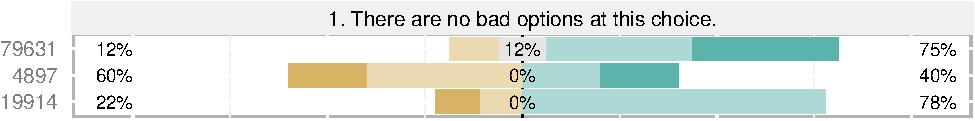
\includegraphics[width=0.485\textwidth]{fig/relaxed-q1.pdf}
  \caption{A graph of responses to question 1 under the ``relaxed'' treatment. The three numbers are the seeds used to generate the three different choices for this treatment. The graph setup is the same as in \cref{fig:report}.}
  \label{fig:relaxedq1}
\end{figure}


The first of our failed hypotheses involved the ``relaxed'' treatment.
%
We expected the ``relaxed'' treatment to elicit agreement with the statement ``There are no bad options at this choice,'' but our statistical test failed to reject the null hypothesis that the answers to this question were consistent with a uniform distribution of underlying responses.
%
A per-choice breakdown of the data for relaxed condition in \cref{fig:relaxedq1} gives a strong indication that the question with seed 4897 elicited qualitatively different responses than the two other questions in this treatment.
%
That particular question is shown in \cref{fig:ch4897}, and reveals one possible reason for what we observed: unlike the other two questions in the ``relaxed'' case, option 3 of this question lists ``no relevant skills'' rather than giving a relevant skill possessed by the player.


\begin{figure}[h]
\fbox{
\parbox{0.95\columnwidth}{
  \slshape
You come to a tavern and decide to rest for a while.
%
A noble is bored and a peasant is bored and a merchant is selling a book of herbal lore.
%
What do you do?
\begin{enumerate}[itemsep=0pt,topsep=4pt,parsep=0pt,partopsep=0pt]
\item You tell the peasant a story \\
  (You have skill: storytelling).
\item You tell the noble a story \\
  (You have skill: storytelling).
\item You offer to trade the merchant your dragon scale for the merchant's book of herbal lore \\
  (no relevant skills).
\end{enumerate}
}
}
  \caption{The ``relaxed'' choice with seed 4897 (minus the framing, which is largely the same as that shown in \cref{fig:exframing}).}
  \label{fig:ch4897}
\end{figure}


The fact that the player doesn't have any skills relevant to that action does not mean that the action will fail, but it might make that option seem less desirable than the others at that choice.
%
None of the options at the other two choices in the ``relaxed'' treatment listed ``no relevant skills,'' they all listed some skill that the player had as relevant, which explains why there might be a difference in responses.
%
If that wording caused the shift, it would be consistent with Schwartz et al.'s theory of satisficing versus maximizing personalities \citep{Schwartz2002}.
%
Schwartz et al. have found that while some people are happy as long as their choices lead to satisfactory results, others are unhappy if their choices lead to good but nevertheless suboptimal results.
%
The strong split in responses for this specific case (including both significant ``strongly disagree'' and significant ``strongly agree'' contingents) indicates that some people may be interpreting the phrase ``bad option'' as meaning options that are absolutely bad, while others may be comparing the options against each other.
%
It would take more data to discern whether this distinction is what is at work here, but it is clear that it is an important distinction for choice poetics, and it is not yet something that \dunyazad/ reasons about.


Although \dunyazad/ does not reason about this, it is to some degree aware of the distinction between the question with seed 4897 and the other two questions in that treatment.
%
The constraints for the ``relaxed'' condition were that each option either ``enables'' or ``achieves'' a goal (in the technical senses; see page \pageref{page:choicetypes}), and in this case, the system generated two options that ``achieved'' a goal and one that merely ``enabled'' a goal, thus creating a distinction even on its own terms.
%
The other two questions in the relaxed category each included three options which ``achieved'' a goal.
%
In light of the survey results, it is clear that to construct choices that unambiguously have ``no bad options'' the system should not only require that each option works towards a player goal, but that each option is balanced against all others.


\subsection{Expectations of Failure}

Another incorrect hypothesis was that in the ``dilemma'' treatment participants would agree with the statement ``All of the options at this choice are about equally promising.''
%
We expected this because one of the constraints of the ``dilemma'' treatment was that all of the threatened goals should have the same priority.
%
However, even for the individual choice in the ``dilemma'' treatment where participants reported the most agreement, 30\% of participants answered ``somewhat disagree.'' 


\begin{figure}[h]
  \includegraphics[width=0.47\textwidth,page=3]{fig/choices-cropped.pdf}
  \caption{A histogram of options selected by participants at the three different ``dilemma'' choices (each labeled by seed).}
  \label{fig:dilchoices}
\end{figure}


\Cref{fig:dilchoices} shows the options that participants said they would choose for the three dilemma choices.
%
For the first two choices, option 2 is a clear loser, and looking at the choices, it's easy to see why.
%
Both of those choices (which are nearly identical) involve being attacked by a dragon.
%
In both choices, option 2 is an option to attack the dragon yourself, but of course you have neither the ``fighting'' skill nor a weapon, and the dragon has both.
%
Although you also lack relevant skills for the other options, making a desperate attempt to flee from or pacify a dragon seems like a better choice than fighting it (at the very least, it did to all of our participants).


The problem here is that the system's representation of player expectations is not fine-grained enough.
%
To the system, all of the options at these choices are expected to ``fail'' the player's goal of keeping their character alive and uninjured, but the system makes no distinction beyond that.
%
How certain does such failure seem to the player?
%
Exactly how badly does the player expect to fare when their goal is not met?
%
In this case, even when told that the situation is hopeless (or perhaps especially then), fleeing seemed a better option than attacking the dragon head-on, but the system doesn't distinguish those cases.
%
Based on this data, the system should be improved by adding more detail to its assessments of goal failure and success.


\subsection{Outcome Clarity}


\begin{figure}[h]
  \hspace*{-0.2em}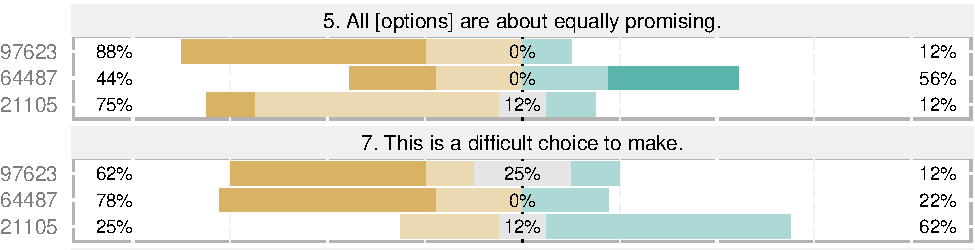
\includegraphics[width=0.485\textwidth]{fig/obvious-q5-q7.pdf}
  \caption{A graph of responses to questions 5 and 7 under the ``obvious'' treatment by seed.}
  \label{fig:obviousq57}
\end{figure}


Although we expected participants to agree that options were balanced for ``dilemma'' choices, we expected them to disagree for ``obvious'' choices.
%
Here again our hypothesis was not supported by our data.
%
A per-choice analysis of question 5 in the ``obvious'' condition (\cref{fig:obviousq57}) shows that again, one choice is divergent from the other two.
%
\Cref{fig:ch64487} shows that choice, which compared to the other two ``obvious'' choices is low-stakes (one of the other choices starts with a dragon attack, the other with bandits attacking some merchants).


Not only are the stakes for this choice low, but they are unclear.
%
What exactly does the player hope to gain by gossiping or by telling a story?
%
Perhaps friendship or some useful information, but those potential rewards seem both uncertain (even given a ``successful'' action) and questionably useful.
%
In contrast (albeit a contrast that participants did not see directly) the utility of fleeing from an attacking monster is clear, even if it is uncertain whether you will succeed.
%
Furthermore, there aren't any obvious risks associated with options 1 and 3, so even if the player is missing a relevant skill, they might still be worth trying.
%
Given this combination of low stakes, a dubious reward for the most-successful-seeming option, and seemingly consequence-free options all around, it is not hard to see how some might find these options ``about equally promising.''


\begin{figure}[h]
\fbox{
\parbox{0.95\columnwidth}{
  \slshape
You come to a tavern and decide to rest for a while.
%
A merchant is bored and a peasant seems knowledgeable and an innkeeper seems knowledgeable.
%
What do you do?
\begin{enumerate}[itemsep=0pt,topsep=4pt,parsep=0pt,partopsep=0pt]
\item You gossip with the innkeeper \\
  (You are missing skill: negotiation).
\item You tell the merchant a story \\
  (You have skill: storytelling).
\item You gossip with the peasant \\
  (You are missing skill: negotiation)
\end{enumerate}
}
}
  \caption{The ``obvious'' choice with seed 64487.}
  \label{fig:ch64487}
\end{figure}


On the other hand, the system's attempt to construct an obvious choice in this case was still mostly successful.
%
7 of 9 participants who saw this choice ``strongly agreed'' with the statement ``There is a clear best option at this choice'' and 8 of those 9 picked option \#2 as the option they would choose.
%
While it might seem like a contradiction to agree (as 3 participants did) with both the statement that a choice has equally promising options and the statement that it has a clear best option, this highlights the difference between outcomes-focused evaluation of individual options and choice-oriented option comparison.
%
The phrasing of ``All of the options at this choice are about equally promising,'' suggests evaluating each option independently and comparing those values roughly.
%
In contrast, ``There is a clear best option at this choice,'' suggests comparing the options against each other to find one that is better than the others.
%
The fact that people often make decisions inconsistent with simple utility calculation is well-known (see e.g., \citep{Tversky1993}), so it should not be surprising that a context in which someone is asked to make a choice might elicit a different response than a context in which someone is asked to rate responses.


\subsection{Conflicting Goals}


\begin{figure}[h]
\fbox{
\parbox{0.95\columnwidth}{
  \slshape
You come across some bandits attacking a merchant.
%
The bandits are threatening the merchant.
%
What do you do?
\begin{enumerate}[itemsep=0pt,topsep=4pt,parsep=0pt,partopsep=0pt]
\item You attack the bandits \\
  (They have skill: fighting. You are missing skill: fighting. They have no tool for fighting).
\item You travel onwards \\
  (no relevant skills).
\item You talk the bandits down \\
  (no relevant skills).
\end{enumerate}
}
}
  \caption{The ``obvious'' choice with seed 21105.}
  \label{fig:ch21105}
\end{figure}


Our hypothesis that respondents would not find ``obvious'' choices difficult highlights a different choice in the ``obvious'' category.
%
Our data did not support this hypothesis, and as shown in \cref{fig:obviousq57}, the choice with seed 21105 accounts for the majority of all responses that contradict our hypothesis.
%
That choice is shown in \cref{fig:ch21105}, and from the system's perspective, it satisfies the definition of an obvious choice (see page \pageref{page:choicetypes}) because the second option ``achieves'' a player goal, while neither the first nor the third do, and both the first and third ``threaten'' a player goal.


The perceived difficulty of this decision probably stems from the fact that it pits two player goals against one another: the goal of self-preservation is best served by option 2, but the goal of helping others in need is best served by one of the other options.
%
Based on this, we plan to change the system's idea of an ``obvious'' choice to better capture these dynamics.
%
Even when one option at a choice clearly has the most-positive outcome for the player considering all goals to be equal, when that choice pits multiple goals against one another, it may be very difficult indeed (this is exactly the form of some morality thought experiments).


However, a detailed inspection of the answer set that resulted in this choice as we were analyzing our data reveals another problem with the system.
%
The system actually thinks that travelling onwards serves the goal of preventing the threat to the merchant (because if the player travels onwards, that entire situation is left behind and therefore the threat no longer exists) while it has no conception that this serves a goal of self-preservation (although it understands that interfering by either means threatens the player's safety).
%
There are thus two more changes to the system prompted by this data: first a bug-fix related to the consequences of travelling onwards, and second, the addition of relative goal relevance across options: the idea that if all but one option threatens an important goal, then the remaining option can be seen as indirectly supporting that goal even if none of its outcomes directly further that goal.
%
Without running this experiment, we would eventually have found and fixed the ``travel onwards'' bug, but we may not have though to make the second change.
%
In this case, our data served to help find and diagnose an anomaly in our system, which turned out to involve both an error in the code, but at the same time also pointed to two positive changes for our choice structure model: adding an explicit notion of goal conflict and a notion of relative goal relevance when all but one option relates to a goal in the same way.

\subsection{Stakes and Consequences}

Our final unsupported hypothesis was that participants would feel more strongly that ``dilemma'' choices had important consequences than that ``obvious'' choices did.
%
This hypothesis was based on the idea that consequences might seem more relevant (and thus important) when a decision was more difficult.
%
Given that one of our ``obvious'' choices seemed difficult to many participants as discussed above, it is unsurprising that this hypothesis was not supported.


\begin{figure}[h]
  \hspace*{-0.2em}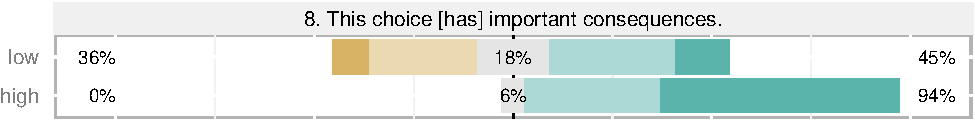
\includegraphics[width=0.485\textwidth]{fig/stakes-q8.pdf}
  \caption{A graph of responses to question 8 across all treatments by question stakes.}
  \label{fig:stakesq8}
\end{figure}


What is interesting is the effect of the choice stakes on this question.
%
Our similar hypothesis that participants would agree more in the ``dilemma'' case than the ``relaxed'' case \emph{was} supported by the data, and one big difference between those two treatments is the stakes associated with them.\footnote{A statistical analysis of the assertion that participants agree more with the statement that a choice's stakes are low in the ``relaxed'' case than the ``dilemma'' case (not one of our original hypotheses) reveals a strong significant effect ($p = 2.88\times10^{-5}$; $r = 53\%$).}
%
In fact, when analyzing the data for question 8 according to stakes rather than the three treatments, high-stakes choices overwhelmingly seem as if they will have important consequences, while low-stakes choices are mixed (see \cref{fig:stakesq8}).


A statistical test confirms the obvious: the high-stakes condition elicits significantly more agreement on question 8 than a uniform distribution ($p = 4.9\times10^{-6}$; $r = 55$\%).
%
Because all of the ``relaxed'' choices were low-stakes by design, there is of course correlation between the stakes and the treatments, but the 35 high-stakes cases were about evenly distributed between the ``obvious'' and ``dilemma'' treatments (16 in ``obvious'' and 19 in ``dilemma'').
%
Such an overwhelming effect (none of the 35 respondents across who saw a high-stakes choices thought it would \emph{not} have important consequences) further indicates that the system is successful in predicting player goals (at least the important player goals): choices where the system thought that an important player goal was affected corresponded almost totally with situations where players felt that consequences were important.


\section{Conclusion}

Overall, our study confirmed \dunyazad/'s ability to construct choices based on player expectations.
%
Notably, many of our failed hypotheses involved situations where several options together affected how a choice was perceived:
%
\begin{itemize}
  \item For question 1 (``There are no bad options at this choice.'') relative rather than absolute judgements of what is a ``bad'' option may have come into play.
  \item For question 5 (``All of the options at this choice are about equally promising.'') it seems \dunyazad/ may need to make finer distinctions between different modes of goal failure, as several options expected to lead to failure may still seem to offer a range of possibilities when no better options are present.
  \item Question 7 (``This is a difficult choice to make.'') showed that a choice can be difficult when multiple goals conflict, even when expectations for one goal are much better than for another.
\end{itemize}
%
These results point to several possible improvements for \dunyazad/, and collectively reinforce the importance of considering choices holistically when evaluating choice poetics.


Based on our results, we plan to upgrade \dunyazad/ in several ways:
%
\begin{itemize}
  \item We plan to implement separate ``satisfaction'' and ``maximization'' player decision modes so that the system can reason about how difficult a decision might seem whichever decision modality a player is using.
  \item We will upgrade \dunyazad/'s system for estimating how individual options affect goals by adding more detail so that it can further distinguish different magnitudes of risk and reward.
  \item We will have \dunyazad/ represent players' uncertainty about the possible outcomes of actions like ``gossip'' and ``tell story'' so that it can have a clearer picture of which options seem promising.
  \item We will implement a model of goal conflicts and more detailed relative goal priorities. This would also allow \dunyazad/ to further support role-playing by allowing different players to choose options which imply different goal priorities.
  \item We will implement the idea of relative goal relevance: if all but one option at a choice either threatens or enables a goal, then the remaining option implicitly does the opposite.
\end{itemize}
%
These changes should make \dunyazad/ even more successful at constructing choices which produce particular player expectations (and thus which can produce specific poetic effects).
%
They are also in line with our goal of getting \dunyazad/ to generate choices with more complex poetics, such as choices that elicit regret or confusion.


Of course, the success of this study can serve as the basis for future studies.
%
One important functionality of \dunyazad/ not tested here was its ability to judge outcomes.
%
Given its player expectations about options (which we now know are often accurate) \dunyazad/ can currently generate outcomes that both support and betray those expectations.
%
Another study could be conducted to test this functionality, as well as some of the choice poetics involved.


Finally, a long-term goal for \dunyazad/ is more player-specific choice generation.
%
Even without running interactively, \dunyazad/ can construct sequences of choices where early choices determine player preferences or behavior and lead to regions of a story with divergent choice structures based on the earlier decisions.
%
Given this kind of capability, \dunyazad/ could not only follow an author's static instructions about what poetics to use, but it could offer choices tailored to players based on the choices they have made.
